\subsubsection{Functional Requirements}
\begin{itemize}
  \item The system must correctly handle the availability of vehicles.
  \item The system must prevent an user from reserving more vehicles.
  \item The system must correctly switch the car state to FREE or RESERVED.
  \item The system must correctly register the reservation's time.
\end{itemize}

\subsubsection{Scenario 1}
After dinner Mark decides to go to the cinema and decides to use a PowerEnJoy's car. He then browses the application and reserves car near him.
Unexpectedly Morgan, a friend of Mark, is having dinner in the same restaurant and when they see each other they start chatting. When they stop talking Mark notices on his PowerEnjoy app that in five minutes his reservation expires. So quickly greets Morgan and goes to unlock his car.

\subsubsection{Scenario 2}
Susan is a typical PowerEnJoy user, she was walking through a street when a friend texts her to hang out. Fortunately she saw a PowerEnJoy's car on the other side of the street. She reached the car and checked online: that's not available. Someone had probably already reserved it. But on the app she noticed that there were two avable car 5 minutes walk from her position. Then she reserved one of that two cars and easily reached it, thanks to the accurate location service provided by the system. 


\subsubsection{Mockups}
\begin{figure}[!ht]
  \centering
  \vspace{0.1cm}
  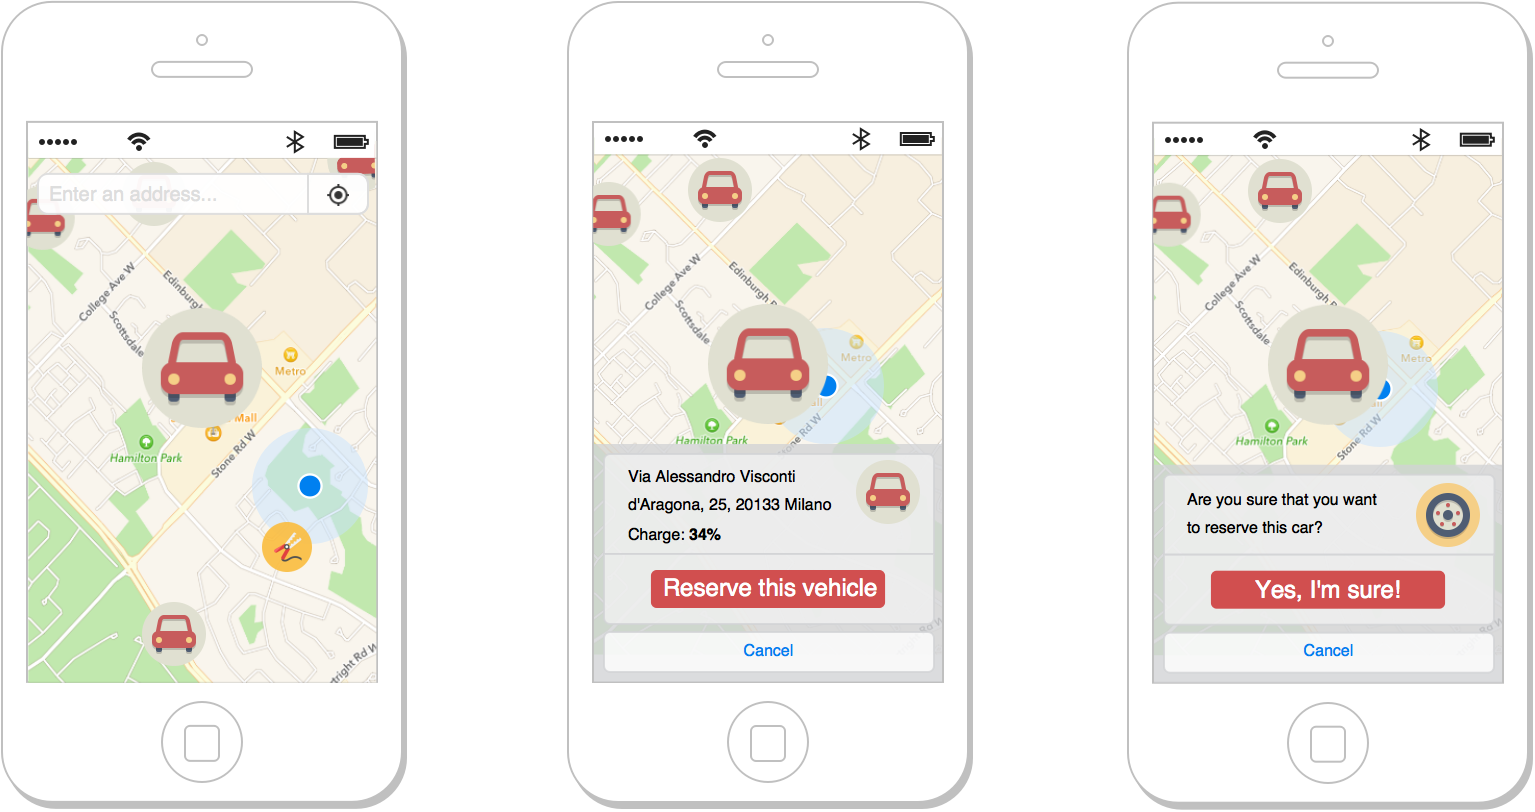
\includegraphics[width=0.9\textwidth]{/RASD/System_Functions/create_reservation_mockup}\\
  \vspace{0.1cm}
  %\caption{Mockup for the login mobile page} 
  \label{fig:create_reservation_mockup} 
\end{figure}
% maybe home page mockup here 


\newpage
\subsubsection{Use-case table}
\begin{center}
  \begin{tabular}{ l | p{10cm} }
    \hline
    Actors & User\\ \hline
    Goal & G\ref{itm:goal-reservation}\\ \hline
    Entry conditions & 
    \begin{itemize}
			\item The User is in his homepage and want to reserve a car.
			\item PowerEnJoy has available cars.
			\item The User is not already reserving a car.
    \end{itemize}  \\ \hline
    Flow of events &
    \begin{itemize}
      \item The user has three ways for finding a car:
      \begin{itemize}
      			\item browse the map.
      			\item use her location.
      			\item enters an address.
      \end{itemize}
      %\item The system loads a map of the selected area and the avaible cars' locations near there .
      \item The user selects the car that want to reserve.
      \item the system displays the car's information.%Maybe to add to the mockup
      %\item The User presses the "Yes,I'm sure" button for confirm the reservation.
      \item The system turns the car "reserved".% and start the reservation timer.
      \item The system notifies the user.
    \end{itemize} \\ \hline
    Exit conditions &
    \begin{itemize}
    	\item A car is set as "reserved".
    	\item The car is reserved for up one hour. After that the reservation expires and the user has to pay a fee of 1eur.
    \end{itemize}  \\ \hline
    Exceptions & 
    \begin{itemize}
    \item The vehicle has already been reserved (the system signals an error).
    \item The system is not able to complete the operation due to some internal issues or connection broken (the system signals a ConnectionFailure).
    \end{itemize}  \\ \hline
  \end{tabular}
\end{center}


\newpage
\subsubsection{Sequence diagram}
\begin{figure}[!ht]
  \centering
  \vspace{0.2cm}
  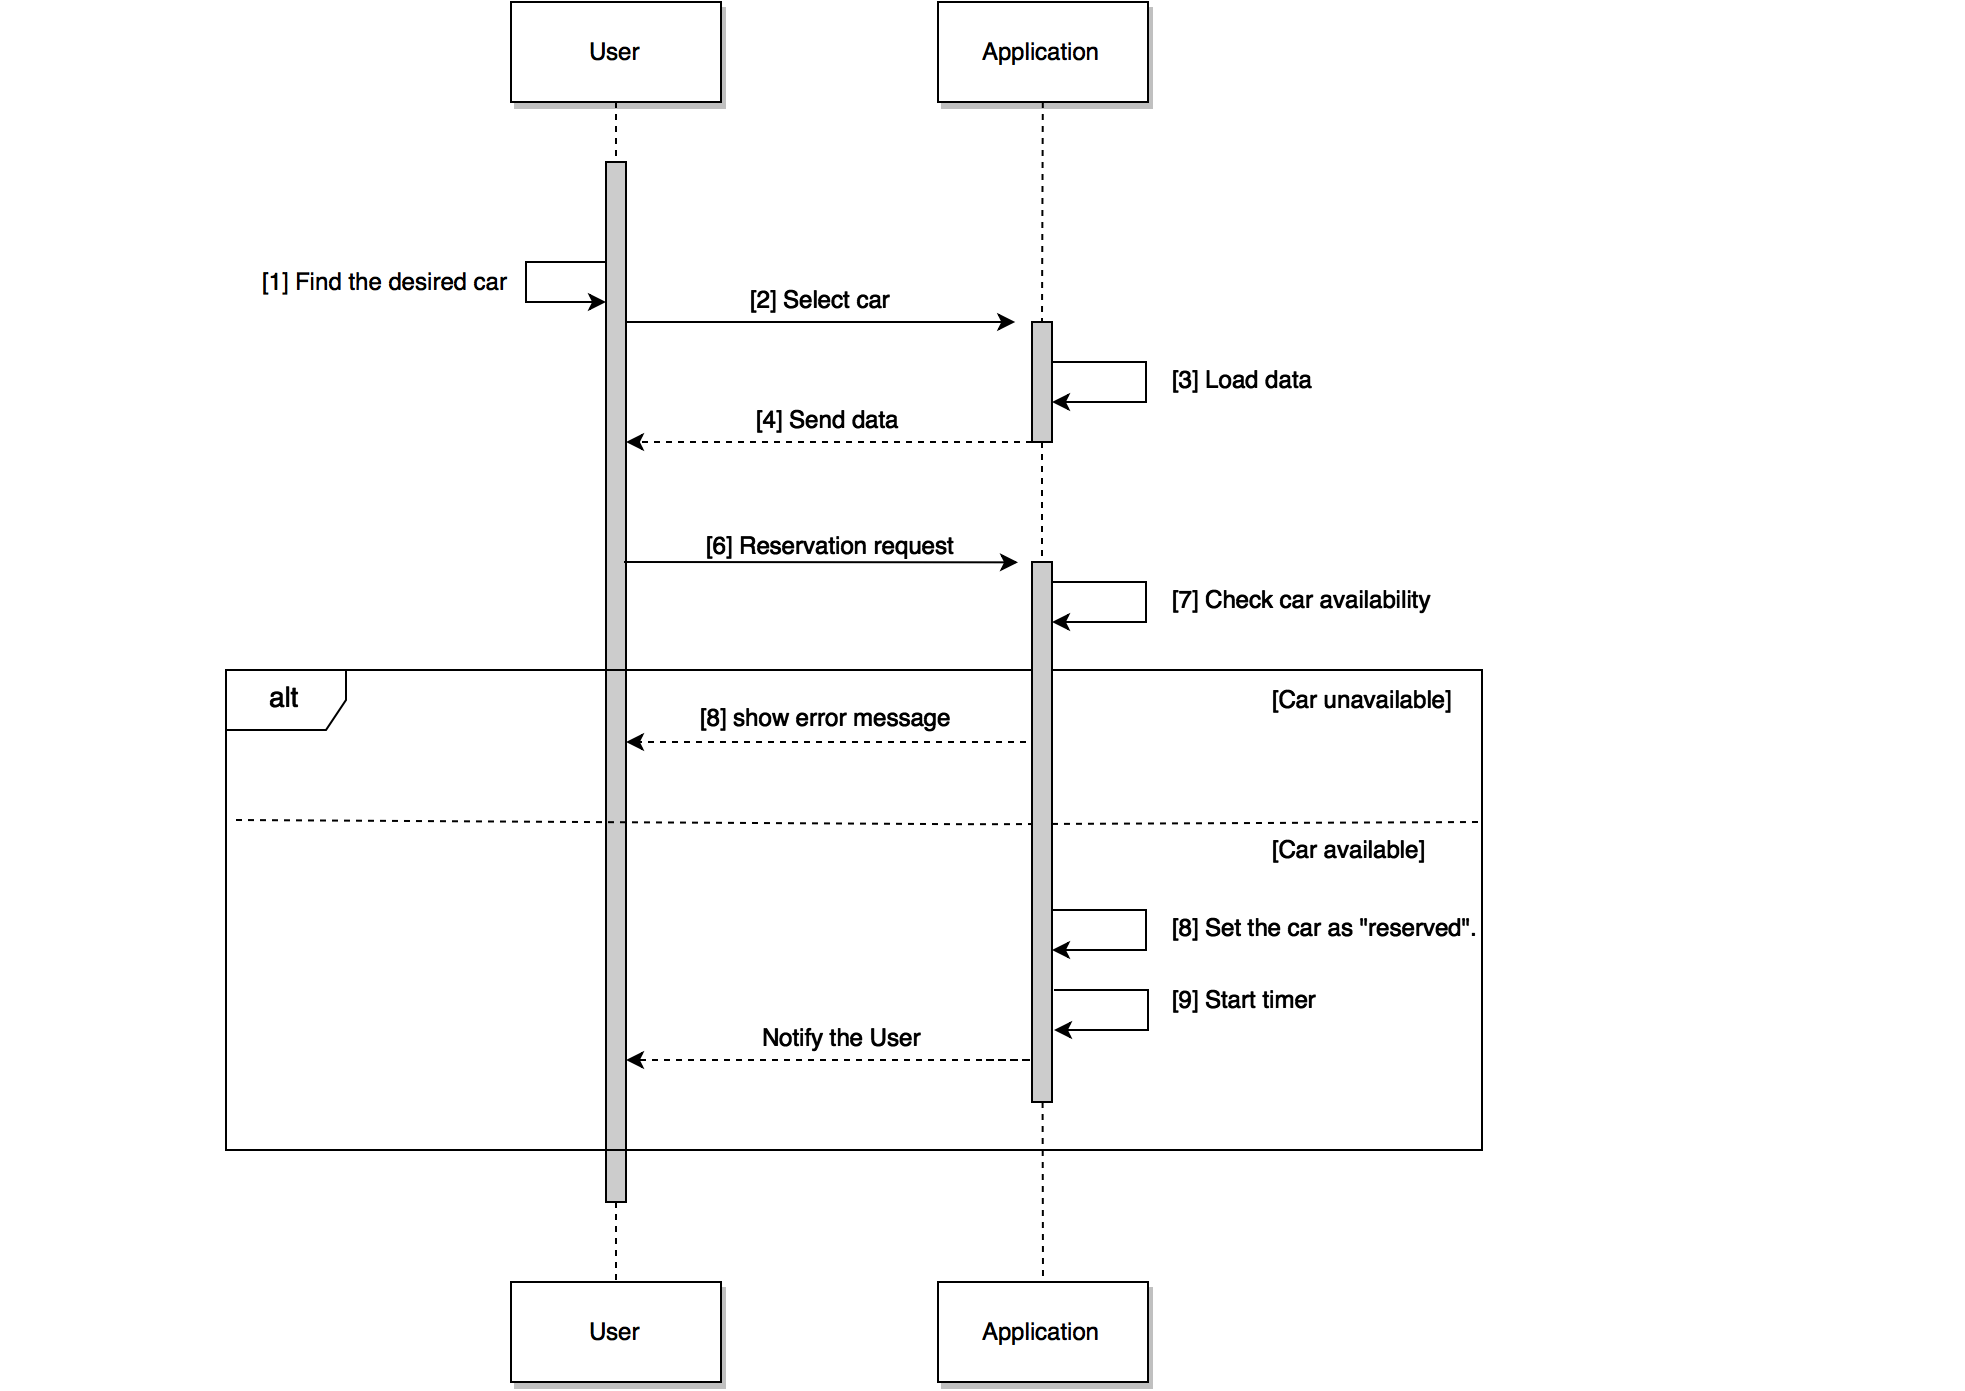
\includegraphics[width=1.1\textwidth]{/RASD/System_Functions/reservation_sequence}\\
  \vspace{0.1cm}
  %\caption{Sequence diagram for the login procedure} 
  \label{fig:reservation_sequence} 
\end{figure}

